\documentclass[a4paper]{article}
\usepackage{exercise}
%um nur aufgaben zu zeigen
%\usepackage[noanswer]{exercise} 
\usepackage{../images/preamble}
\usepackage{rotating}
\usetikzlibrary{decorations.pathmorphing}
\usetikzlibrary{decorations.markings}
\usetikzlibrary{arrows}
\usetikzlibrary{shapes.geometric}
\newcommand{\midarrow}{\tikz \draw[-triangle 90] (0,0) -- +(.02,0);}
\usepackage{xcolor}
%\usepackage{draftwatermark}
%\SetWatermarkText{\textsc{Entwurf}}
%\SetWatermarkScale{6}
%\SetWatermarkColor{red!30}




\begin{document}
	\vspace*{-2cm}
	\parbox{4cm}{
\includegraphics[width=2.5cm]{../images/ROLF4.png}}
	\parbox{10.6cm}{\setstretch{2.0} \centering{ \huge \textsf{Aufgabenseminar Himmelsmechanik
				}}\\
\href{mailto:physikrolf@gmail.com}{physikrolf@gmail.com}, \url{pankratius.github.io/rolf} \\ \vspace*{-.5cm} }
	
	

\thispagestyle{empty}
%\begin{framed}
%	\noindent
%	\scriptsize
%	Die Aufgaben sollten bis zum \textbf{5. Oktober} bearbeitet werden. Die Lösungen schickt ihr an .
%	Jede Aufgabe hat eine bestimmte Anzahl an erreichbaren Punkten. Wie viele das sind, müsst ihr raten. Versucht, die Lösungen so genau wie möglich aufzuschreiben. Für besonders schnelle/gute/witzige Lösungen kann es Bonuspunkte geben.\\ Die aktuellen Aufgaben sowie alle alten Aufgabenserien mit Lösungen findet ihr auch auf \url{pankratius.github.io/rolf}. %\\\textit{Zu jeder Aufgabe gibt es jetzt Tipps. Die sollten beim Lösen der Aufgaben helfen.\\ Sollte das so sein macht bitte in euren Lösungen kenntlich, dass bestimmte Schritte von den Tipps und nicht von euch kommen. Darauf gibt es keinen Abzug, es ist nur für uns gut zu wissen.}
%\end{framed}

\noindent

\begin{minipage}[b]{0.65\textwidth}
\begin{Exercise}[title = Polygon, origin = P. Gnädig, difficulty = 2, label = polygrav]
	Wir betrachten ein regelmäßiges n-Eck, bei dem an jeder Ecke eine Masse $m$ sitzt. Wie bewegt sich das System, wenn nur die Gravitationskraft zwischen den Körpern wirkt? Wie viel Zeit (in Abhänigkeit von $n$) vergeht, bis das System seinen Endzustand erreicht hat? 
\end{Exercise}
\end{minipage}
\begin{minipage}[b]{0.35\textwidth}
	\centering
	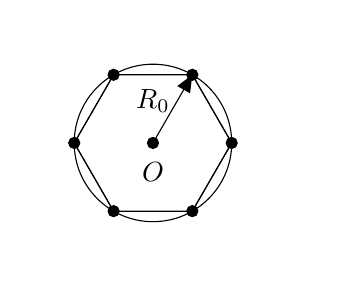
\begin{tikzpicture}[line cap=round,line join=round,>=triangle 45,x=1.0cm,y=1.0cm]
	\clip(-1.0911274272504616,-0.595261736026898) rectangle (2.4959243296533993,2.330040817448145);
	\draw(0.,0.) -- (1.,0.) -- (1.5,0.8660254037844387) -- (1.,1.7320508075688776) -- (0.,1.7320508075688779) -- (-0.5,0.8660254037844395) -- cycle;
	\draw (0.,0.)-- (1.,0.);
	\draw (1.,0.)-- (1.5,0.8660254037844387);
	\draw (1.5,0.8660254037844387)-- (1.,1.7320508075688776);
	\draw (1.,1.7320508075688776)-- (0.,1.7320508075688779);
	\draw (0.,1.7320508075688779)-- (-0.5,0.8660254037844395);
	\draw (-0.5,0.8660254037844395)-- (0.,0.);
	\draw(0.5,0.866025403784439) circle (1.cm);
	\draw [->] (0.5,0.866025403784439) -- (1.,1.7320508075688776);
	\begin{scriptsize}
	\draw [fill=black] (0.,0.) circle (2.0pt);
	\draw [fill=black] (1.,0.) circle (2.0pt);
	\draw [fill=black] (1.5,0.8660254037844387) circle (2.0pt);
	\draw [fill=black] (1.,1.7320508075688776) circle (2.0pt);
	\draw [fill=black] (0.,1.7320508075688779) circle (2.0pt);
	\draw [fill=black] (-0.5,0.8660254037844395) circle (2.0pt);
	\draw [fill=black] (0.5,0.866025403784439) circle (2.0pt);
	\end{scriptsize}
	\node at (0.5,1.4){$R_0$};
	\node at (0.5,0.5){$O$};
	\end{tikzpicture}
\end{minipage}
\begin{Answer}[ref = polygrav]
	Aus Symmetriegründen heben sich die nicht-radialen Teile der wirkenden Gravitationskräfte auf, sodass alle $n$ Massen sich zum Mittelpunkt des Polygons, $O$, bewegen. Dabei muss die polygonform erhalten bleiben. Weil die Abhängigkeit Körperabstand-Gravitationskraft aber nicht-linear ist, ist die Bewegung nicht gleichmäßig beschleunigt. Vielmehr sollte die Beschleunigung größer werden, je geringer der Körperabstand ist.\\
	Um nun die Zeit $T$ auszurechnen, bis die Körper im Punkt $O$ kollidieren, kann man zuerst die Kraft auf eine der Massen $m$ ausrechnen. Diese ist gegeben durch die Summe der Radialteile aller  Gravitationskräfte der anderen $n-1$ Körper, also, wenn der Radius des Polygons gerade $R$ ist,
	\begin{equation}\label{polygrav:f}
		F = Gm \sum_{i= 1}^{n-1}\frac{m \sin\left(\frac{\pi}{i}\right)}{\left(2R  \sin\left(\frac{\pi}{i}\right)\right)^2} = \frac{Gm}{R^2}\cdot \underbrace{ \frac{m}{4}\sum_{i=1}^{n-1} \frac{1}{\sin \frac{\pi}{i}}}_{:= M_n}.
 	\end{equation}
 	Die Kraft ist also so, als würde sich der Körper im Gravitationsfeld eines stationären Körpers mit der Masse $M_n = \frac{m}{4}\sum_{i=1}^{n-1} \frac{1}{\sin \frac{\pi}{i}}$ bewegen.\\
 	Diese Bewegung kann man jetzt als Bewegung entlang einer Ellipse ohne kleiner Halbachse, und mit großer Halbachse $\frac{R_0}{2}$ auffassen. Die Zeit, die dann bis zum Zusammensturz benötigt wird, entspricht genau der halben Periode $\nicefrac{T_e}{2}$. \\
 	Diese kann man über das dritte Keplersche Gesetz aus der entsprechenden Periode $T_k$ für eine Kreisbahn mit Radius $R_0$ ausrechen, wobei $F_g = F_{rad}$ benutzt wird:
 	\begin{equation}\label{polygrav:tc}
 		\frac{GmM_n}{R_0^2}  = m R\underbrace{\left(\frac{2\pi}{T_k}\right)^2}_{=\omega ^2} \Rightarrow T_k = 2\pi\sqrt{\frac{R_0^3}{GM_n}}.
 	\end{equation}
 	Mit dem dritten Keplerschen Gesetz folgt dann
 	\begin{equation}
 	\boxed{	\left(\frac{T_e}{T_k}\right)^2 = \left(\frac{\nicefrac{R_0}{2}}{R_0}\right)^3 \Rightarrow T_e = \pi \sqrt{\frac{R_0^3}{8GM_n}}.}
 	\end{equation}
\end{Answer}
 



\end{document}
